
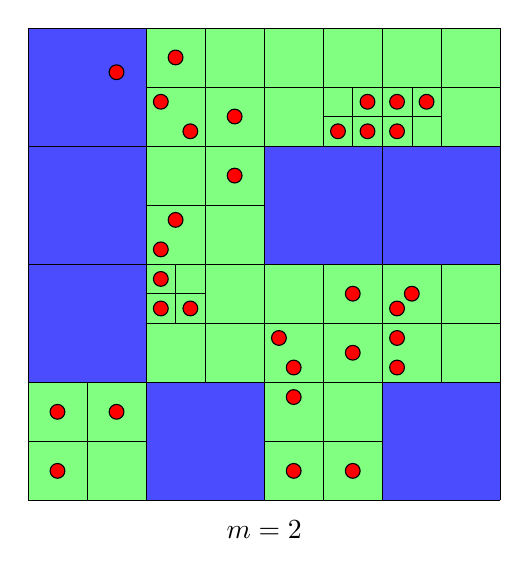
\begin{tikzpicture}[scale=0.75]

				\fill[blue!70] (2,0) rectangle (4,2);
				\fill[blue!70] (0,2) rectangle (2,8);
				\fill[blue!70] (4,4) rectangle (8,6);
				\fill[blue!70] (6,0) rectangle (8,2);
				
 				\fill[green!50] (0,0) rectangle (2,2); 				
 				\fill[green!50] (2,2) rectangle (4,8);
 				\fill[green!50] (4,0) rectangle (6,4);
 				\fill[green!50] (6,2) rectangle (8,4);
 				\fill[green!50] (4,6) rectangle (8,8);
	  		
	  		%% points ...	  		
	  		\draw[fill=red] (2.25,3.75) circle (0.125);
	  		\draw[fill=red] (2.25,3.25) circle (0.125);
	  		\draw[fill=red] (1.5,1.5) circle (0.125);
	  		\draw[fill=red] (0.5,1.5) circle (0.125);	
	  		
	  		\draw[fill=red] (4.5,0.5) circle (0.125);
	  		\draw[fill=red] (5.5,0.5) circle (0.125);
	  		\draw[fill=red] (5.5,2.5) circle (0.125);
	  		\draw[fill=red] (5.5,3.5) circle (0.125);	  		
	  		\draw[fill=red] (6.5,3.5) circle (0.125);
	  		
	  		
	  		\draw[fill=red] (3.5,5.5) circle (0.125);
	  		\draw[fill=red] (3.5,6.5) circle (0.125);
	  		\draw[fill=red] (2.5,7.5) circle (0.125);
	  		
	  		\draw[fill=red] (6.25,6.25) circle (0.125);
	  		\draw[fill=red] (6.75,6.75) circle (0.125);
	  		\draw[fill=red] (5.25,6.25) circle (0.125);
	  		\draw[fill=red] (5.75,6.75) circle (0.125);

        \draw[fill=red] (0.5, 0.5) circle (0.125);
	  		\draw[fill=red] (1.5, 7.25) circle (0.125);	  		
	  		\draw[fill=red] (2.25, 4.25) circle (0.125);
	  		\draw[fill=red] (2.5,4.75) circle (0.125);
	  		\draw[fill=red] (2.75, 3.25) circle (0.125);
	  		\draw[fill=red] (4.5, 1.75) circle (0.125);
	  		\draw[fill=red] (2.75, 6.25) circle (0.125);
	  		\draw[fill=red] (4.25, 2.75) circle (0.125);
	  		\draw[fill=red] (6.25,2.75) circle (0.125);
	  		\draw[fill=red] (6.25,2.25) circle (0.125);
	  		\draw[fill=red] (6.25,3.25) circle (0.125);
	  		\draw[fill=red] (5.75,6.25) circle (0.125);
	  		\draw[fill=red] (6.25,6.75) circle (0.125);
	  		\draw[fill=red] (2.25,6.75) circle (0.125);
	  		\draw[fill=red] (4.5,2.25) circle (0.125);
	  		  		
	  		
				\draw (4,-0.5) node {$m = 2$};

	    	% domain boundary 
	  		\draw[black, very thin, step=2] (0,0) grid (8,8);
	  		\draw[black, very thin, step=1] (0,0) grid (2,2);
	  		\draw[black, very thin, step=1] (2,2) grid (4,4);
	  		\draw[black, very thin, step=1] (4,0) grid (6,4);
	  		\draw[black, very thin, step=1] (6,2) grid (8,4);
	  		\draw[black, very thin, step=1] (2,4) grid (4,8);
	  		\draw[black, very thin, step=1] (4,6) grid (8,8);
	  		\draw[black, very thin, step=0.5] (2,3) grid (3,4);
	  		\draw[black, very thin, step=0.5] (5,6) grid (7,7);

	  		
   	\end{tikzpicture}  